\documentclass[10pt,a4paper]{article}
\usepackage[margin=1.4cm]{geometry}
\usepackage[T1]{fontenc}
\usepackage{lmodern}
\usepackage{helvet}                 % clean sans-serif for a resume artifact
\renewcommand{\familydefault}{\sfdefault}
\usepackage{xcolor}
\usepackage{booktabs}
\usepackage{array}
\usepackage{tabularx}
\usepackage{enumitem}
\usepackage{tikz}
\usetikzlibrary{positioning,arrows.meta}
\usepackage[colorlinks=true]{hyperref}

\definecolor{ink}{RGB}{25,30,40}
\definecolor{brand}{RGB}{10,70,150}
\definecolor{accent}{RGB}{0,120,120}
\definecolor{good}{RGB}{20,110,40}
\definecolor{soft}{RGB}{90,100,115}
\definecolor{band}{RGB}{235,242,250}
\definecolor{chip}{RGB}{225,236,248}

\hypersetup{linkcolor=brand, urlcolor=accent, pdftitle={FPGA Tick-to-Trade Engine}}
\setlength{\parindent}{0pt}
\setlength{\parskip}{3pt}
\renewcommand{\arraystretch}{1.15}
\pagestyle{empty}
\color{ink}

\newcommand{\dsec}[1]{\vspace{4pt}{\color{brand}\large\bfseries #1}\\[-5pt]
  {\color{brand!30}\rule{\linewidth}{1pt}}\\[1pt]}
\newcommand{\chip}[1]{\tikz[baseline=-0.6ex]{\node[fill=chip,rounded corners=2pt,inner sep=2.4pt,font=\footnotesize]{#1};}}
\newcommand{\metric}[2]{\begin{minipage}[t]{0.235\linewidth}\centering
  {\color{brand}\bfseries\large #1}\\[-1pt]{\footnotesize\color{soft} #2}\end{minipage}}

\begin{document}

% ───────────────── Header ─────────────────
{\Huge\bfseries\color{ink} FPGA Tick-to-Trade Engine}\\[2pt]
{\large\color{accent} A nanosecond-latency, fully-pipelined hardware trading datapath for NASDAQ market data}\\[5pt]
{\footnotesize\color{soft}
\chip{SystemVerilog} \chip{Xilinx UltraScale+} \chip{Vivado (synth + P\&R)} \chip{cocotb / Python}
\chip{AXI4-Stream / AXI4-Lite} \chip{NASDAQ ITCH 5.0} \chip{fixed-point DSP}}

\vspace{6pt}
{\color{band}\rule{\linewidth}{18pt}}\\[-15pt]
\hspace*{0.0\linewidth}%
\metric{205\,ns}{tick-to-trade latency}\hfill
\metric{0\,ns}{jitter (deterministic)}\hfill
\metric{200\,MHz}{timing-closed (WNS\,$>$\,0)}\hfill
\metric{200\,MB/s}{line-rate ITCH ingest}
\\[8pt]

% ───────────────── Overview ─────────────────
\dsec{Overview}
An end-to-end high-frequency-trading pipeline implemented entirely in FPGA fabric: it
ingests a raw NASDAQ \textbf{ITCH 5.0} byte stream, maintains a live \textbf{limit order
book}, computes a depth-weighted \textbf{imbalance trading signal}, applies
\textbf{pre-trade risk checks}, and emits an order decision in a fixed
\textbf{205\,ns} (41 clock cycles at 200\,MHz). The datapath is a deeply pipelined
spatial dataflow with \textbf{zero floating-point} and a hardware latency counter for
self-measurement. A bit-accurate Python model mirrors the hardware exactly, serving
both as the verification golden reference and as the software performance baseline.

% ───────────────── Architecture ─────────────────
\dsec{Architecture --- 5-stage hardware pipeline}
\vspace{2pt}
\begin{center}
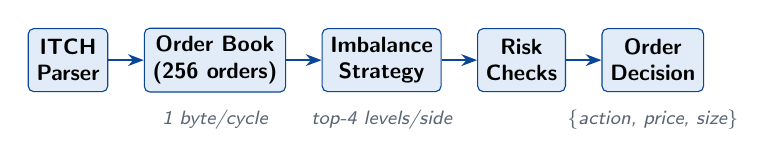
\begin{tikzpicture}[node distance=4.5mm,
  b/.style={draw=brand,fill=chip,rounded corners=2pt,minimum height=8mm,
            align=center,font=\footnotesize\bfseries,inner sep=3pt},
  a/.style={-{Stealth[length=2mm]},brand,thick}]
  \node[b] (p) {ITCH\\Parser};
  \node[b,right=of p] (o) {Order Book\\(256 orders)};
  \node[b,right=of o] (s) {Imbalance\\Strategy};
  \node[b,right=of s] (r) {Risk\\Checks};
  \node[b,right=of r] (d) {Order\\Decision};
  \draw[a] (p)--(o); \draw[a] (o)--(s); \draw[a] (s)--(r); \draw[a] (r)--(d);
  \node[font=\scriptsize\itshape,soft,below=1mm of o] {1 byte/cycle};
  \node[font=\scriptsize\itshape,soft,below=1mm of s] {top-4 levels/side};
  \node[font=\scriptsize\itshape,soft,below=1mm of d] {\{action, price, size\}};
\end{tikzpicture}
\end{center}
\vspace{-2pt}
Streams 1 ITCH byte per clock; a 256-slot direct-mapped order table with a sorted
top-4-levels-per-side cache; depth-weighted imbalance signal with spread guard and
imbalance-scaled lot sizing; priority-encoded risk engine (order-size, price-band, net
position, kill-switch). Host I/O over AXI4-Stream (data) and AXI4-Lite (control + on-chip
latency histogram readout).

% ───────────────── Results ─────────────────
\dsec{Results \& performance vs. software}
\begin{tabularx}{\linewidth}{@{}lXr@{}}
\toprule
\textbf{Metric} & \textbf{Detail} & \textbf{Value} \\
\midrule
Tick-to-trade latency   & 41 cycles @ 200\,MHz, parse-to-decision           & \textbf{205\,ns} \\
Determinism             & fixed-latency pipeline, no caches/OS/scheduler     & \textbf{0\,ns jitter} \\
Speed-up vs optimized C & same computation, median (compiled \texttt{-O2})   & \textbf{$\sim$5$\times$} \\
Tail-latency advantage  & CPU spikes to $\sim$1\,ms; FPGA fixed at 205\,ns   & \textbf{up to $\sim$1{,}800$\times$} \\
Throughput              & 1 byte/cycle ITCH ingest                           & \textbf{200\,MB/s} \\
Timing closure          & Vivado P\&R, UltraScale+, positive worst slack     & \textbf{200\,MHz} \\
Logic footprint         & single-symbol engine                               & \textbf{$\sim$7K LUTs} \\
ITCH message types      & A, F, C, D, E, U, X, P                              & \textbf{8 decoded} \\
\bottomrule
\end{tabularx}

% ───────────────── Verification ─────────────────
\dsec{Verification \& engineering rigor}
\begin{itemize}[leftmargin=1.2em,itemsep=1pt,topsep=1pt]
  \item \textbf{81/81} cocotb tests passing; every RTL block diffed against a
        bit-accurate Python golden model on large synthetic and replayed ITCH streams.
  \item \textbf{Latency self-measured} on-chip (cycle-accurate counter, read over
        AXI4-Lite) and corroborated by Vivado static timing analysis.
  \item Software baselines (compiled C and Python) implemented for an apples-to-apples
        latency comparison of the identical computation; SystemVerilog assertions and
        back-pressure no-drop checks across the pipeline.
\end{itemize}

\vfill
{\footnotesize\color{soft} Implemented in SystemVerilog; synthesized and place-\&-routed in Vivado on a
Xilinx UltraScale+ FPGA; verified with cocotb against a Python golden model.}

\end{document}
